\section{MLP}
\begin{frame}[c]{Multi-Layer Perceptron}
    \begin{figure}
        \captionsetup[subfigure]{labelformat=empty, font={color=black}}
        \begin{subfigure}{0.6\textwidth}
            % trim=left bottom right top, clip
            \centering
            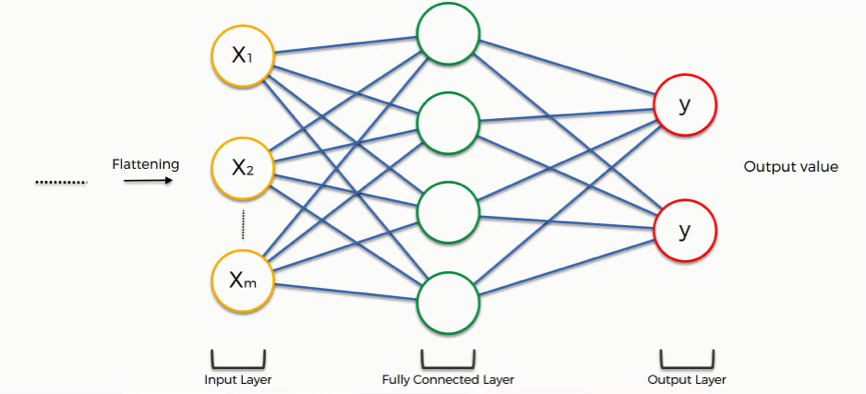
\includegraphics[width=0.7\textwidth,trim=90 0 60 0,clip]{dense_layer}
            \caption{\gls{MLP} with one fully connected layer. Alternative names include 'dense', 'fully connected' and 'mlp' layer. Figure from \cite{convolutional_2018}.}
        \end{subfigure}
        \hspace{3em}
        \begin{subfigure}{0.3\textwidth}
            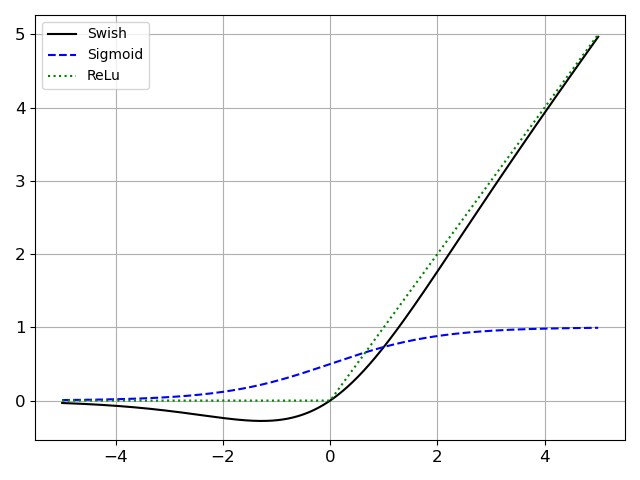
\includegraphics[width=\textwidth]{sigmoid_swish_relu}
            \caption{Common activation function: \gls{ReLU}, or recently for \glspl{LLM}: \gls{SwiGLU}.}
        \end{subfigure}
    \end{figure}
\end{frame}

\section{Training LLMs}
\begin{frame}[c]{InstructGPT: Following Instructions}
    \large
    \begin{aquote}{Ouyang et. al. 2022 \cite{ouyang_training_2022}}
        In human evaluations on our prompt distribution, outputs from the 1.3B
        parameter InstructGPT model are preferred to outputs from the 175B
        GPT-3, despite having 100x fewer parameters. Moreover, InstructGPT
        models show improvements in truthfulness and reductions in toxic output
        generation while having minimal performance regressions on public NLP
        datasets.
    \end{aquote}
    \pnote{
        You had to write 'a good list of .... would be:' before that
    }
\end{frame}

\begin{frame}[c]{Reinforcement Learning from Human Feedback}
    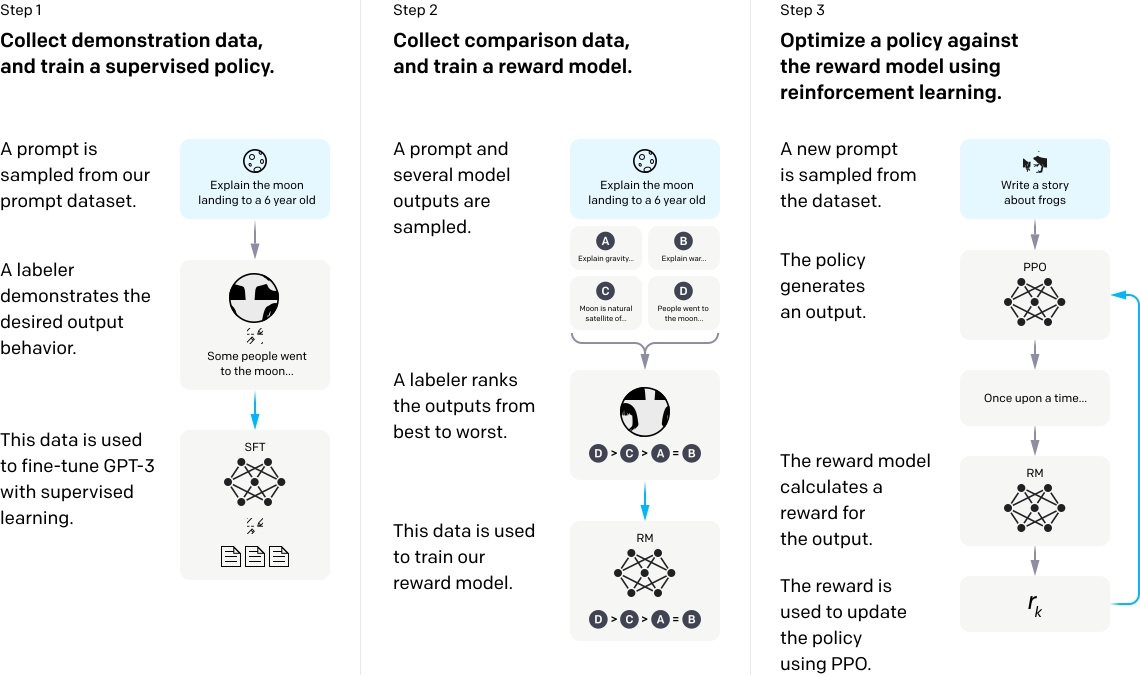
\includegraphics[height=0.7\textheight]{instruct}\\
    \gray{Image Source: \cite{ouyang_training_2022}} \large \hspace{2em} RLHF originated from \cite{christiano_deep_2017}
\end{frame}

\begin{frame}[c]{ChatGPT}
    
\includegraphics[height=0.7\textheight]{chatgpt} \\
    \gray{Image Source: \cite{chatgpt_2023}}
\end{frame}

\begin{frame}[c]{ChatGPT Training Steps}
    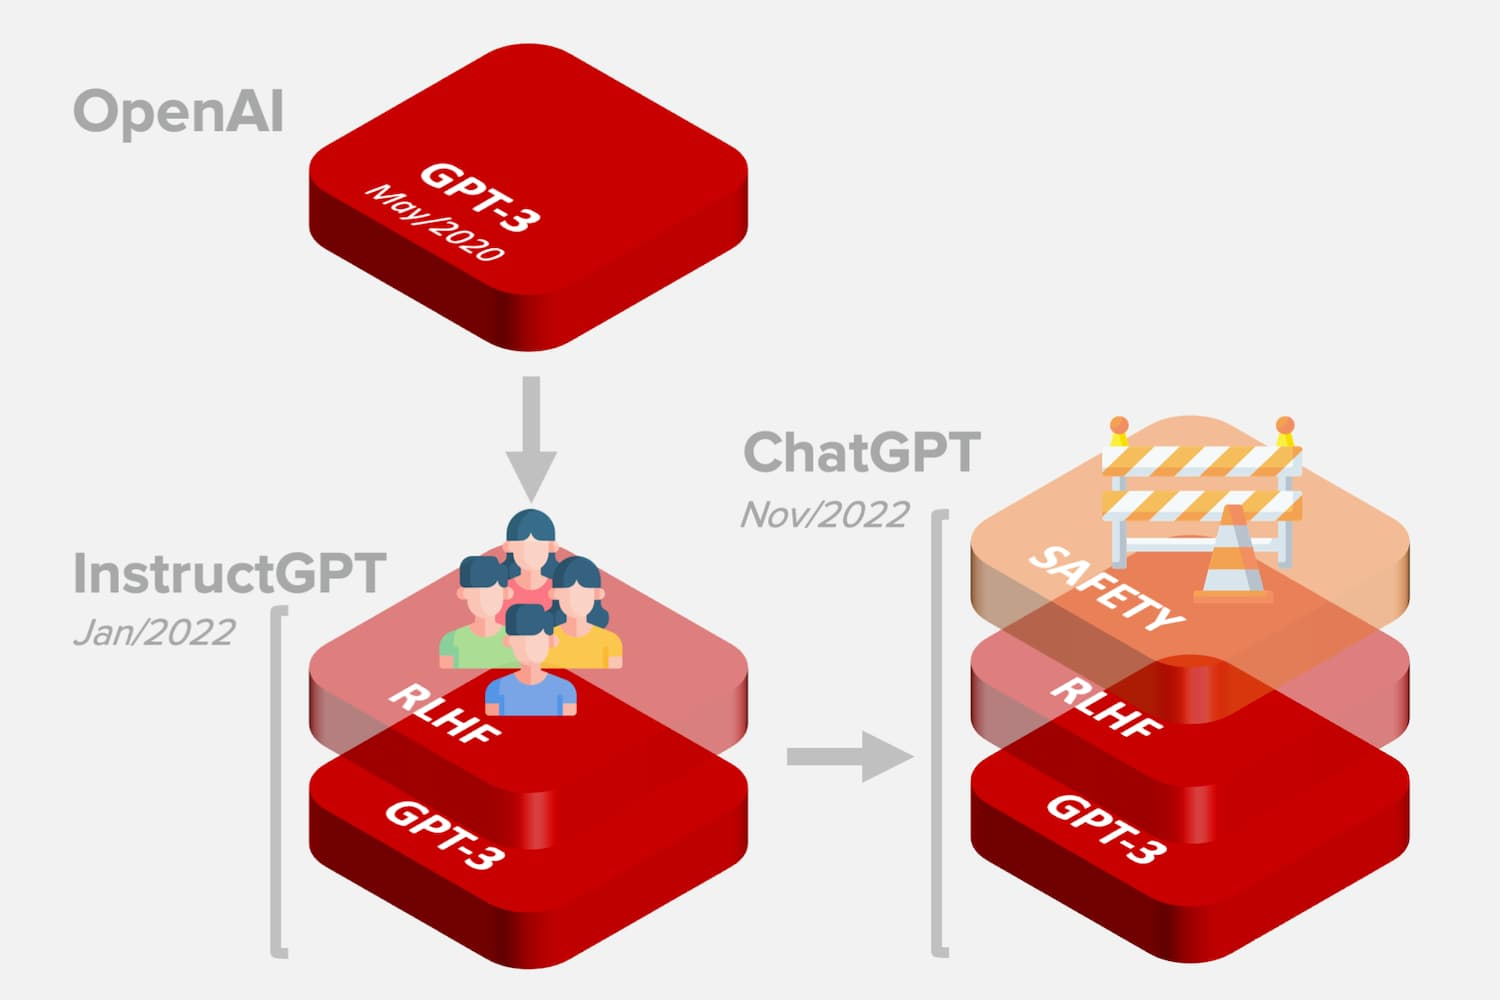
\includegraphics[height=0.7\textheight]{chat_instruct} \\
    \gray{Image Source: \cite{what_2023}}
    \pnote{
        Technically speaking often Instruct=RLHF but eh\\
        \\
        ChatGPT is thus a 'lobotomized', \\
        less useful version when compared to the original InstructGPT
    }
\end{frame}

\begin{frame}[c]{Constitutional AI}
    \large
    \begin{enumerate}[<+(1)->]
        \item Prompt LLM with questions illiciting ethically questionable responses
        \item Ask it to "rewrite this to be more ethical"
        \item Fine-Tune to prefer rewritten response
        \item Repeat a few times
    \end{enumerate}
\end{frame}

\begin{frame}[c]{Constitutional Results}
    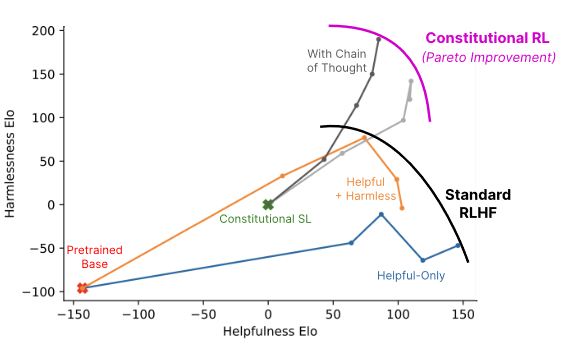
\includegraphics[height=0.7\textheight]{constitutional_benchmark} \\
    \gray{Image Source: \cite{bai_constitutional_2022}}
    \pnote{
        The model uses the ethics it learned implicitly. \\
        Not sure if this creates additional problems
    }
\end{frame}
